\cleardoublepage

\chapter{Comparison to the Previous Version of the Framework}
\begin{figure}[H]
    \centering
    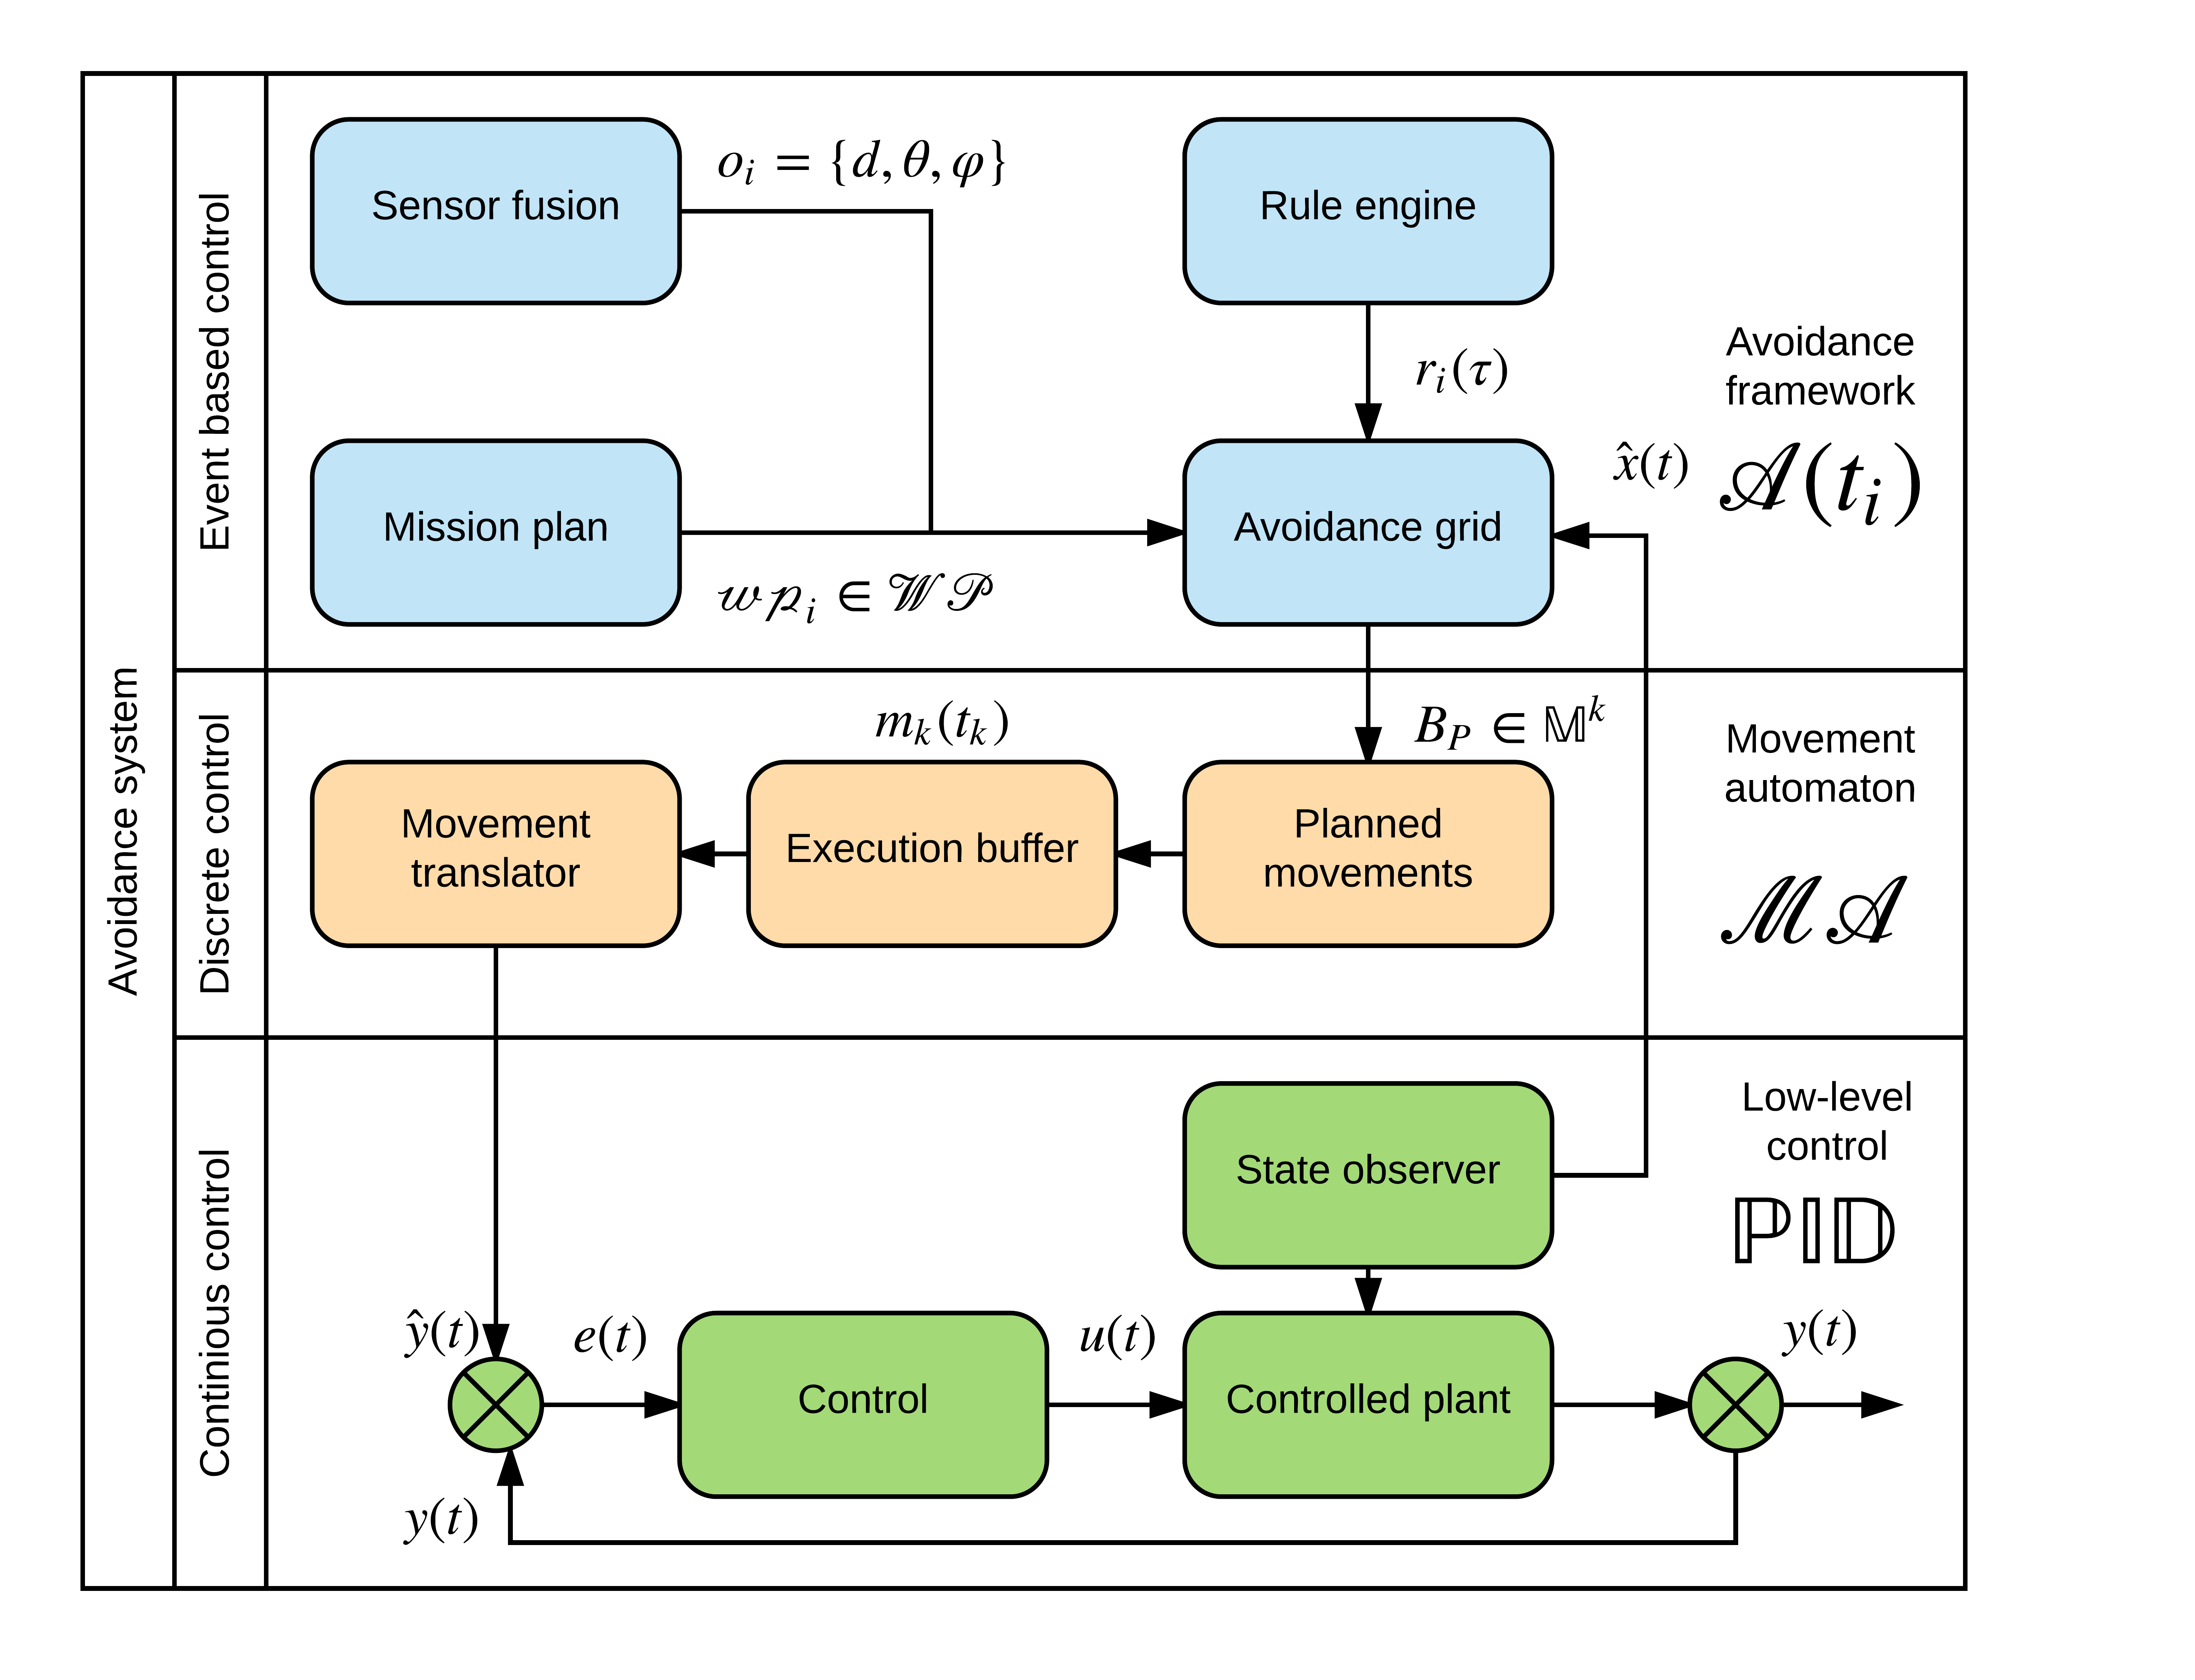
\includegraphics[width=0.8\linewidth]{\FIGDIR/TE001BlockSchemeOfControlConcept} 
    \caption{Obstacle avoidance based on Reach sets concept \cite{gomola2017obstacle}.}
    \label{fig:avoidanceConcept}
\end{figure}

\paragraph{Conceptual scheme:} The overall concept of \emph{Detect and Avoid Framework} (fig. \ref{fig:avoidanceConcept}) is taking architecture from LSTS toolchain \cite{pinto2013lsts,pinto2012implementation}. The UAS part is based on \emph{LSTS Dune}, and it can be easily integrated in the future. 

\begin{enumerate}
    \item \emph{Continuous control} - is not solved in this work, its kept in the scheme for reference. 
    
    \item \emph{Discrete control} - it bridges event based \emph{Detect \& Avoid} core functionality with \emph{Continuous control}. Its covered by \emph{Movement Automaton} (sec. \ref{s:movementAutomatonTheory}).

   
    \item \emph{Event-based control} - covers major functionalists:    
    \begin{enumerate}[a.]
        \item \emph{Sensor (Data) fusion} - the main feed of information, implementation of \emph{sensor fusion} (sec. \ref{s:SensorFusionDefinition}) and \emph{data fusion} (sec. \ref{s:dataFusionDefinition}) contributing the avoidance events, introduced in (sec. \ref{s:dataFusionProbabilisticModelTheory}).
        
        \item \emph{Mission plan} - feeding actual goal and objectives to \emph{Navigation Algorithm} (sec. \ref{s:NavigationAlgorithms}) and obeying \emph{UTM directives} (sec. \ref{s:utmServicesTheory}).
        
        \item \emph{Avoidance Grid}  - using mainly \emph{Approximation of Reachable Space} (sec. \ref{s:ReachSetEstimationTheory}) in \emph{Avoidance Maneuver Estimation}.
        
        \item \emph{Rule engine} - enforcing UTM directives (sec. \ref{s:utmServicesTheory}).
    \end{enumerate}
    
\end{enumerate}

\paragraph{Surveillance Improvements in Our Work:}

\emph{Hierarchical calculation} is addressed in \emph{Mission Control run} (sec: \ref{s:missionControlRun}) where threats are hierarchically applied based on \emph{severity}.

\emph{Source reliability evaluation} is addressed in \emph{Static Obstacles} (sec. \ref{s:staticObstacles}) and \emph{Moving Obstacles} \ref{s:intruders}). The main rating for \emph{Detected obstacle, Map Obstacle} and \emph{Visibility} of space are established there. 

\emph{Clear rating definition} - the \emph{Reachability} of space portion and \emph{Safety} rating for trajectory are established in \emph{Avoidance Grid Run} (sec. \ref{s:aviudabceGridRun})

\paragraph{Reach Set Improvements in Our Work:}

\emph{Limited system dimension} - the discretization due to the higher system dimension and  increased maneuver complexity goes hand-in-hand with \emph{pre-calculation} of the \emph{Reach Set}. This shortcoming is addressed in (sec. \ref{s:constrainedTrajectoryExpansion}).

\emph{Real-time optimization} -  replaced by \emph{Discrete offline optimization problem}. The \emph{general cost function} is given in (eq. \ref{eq:costFunctionReachable}). The optimization problem solved in this work is defined in (eq. \ref{eq:trajectoryTrackingOptimalizaitonProblem}).

\emph{Continuous space disparity} - The \emph{pre-calculated reach set estimation} can be valid with a small \emph{marginal error} for some region in \emph{system state space}. The dynamic method for state space segmentation can be used \cite{takahashi1996reasonable}. This aspect is not addressed in this work, because it strongly depends on the system behind movement automaton. 

\emph{Trajectory Tracking} - The \emph{movement automaton} (def. \ref{def:movementAutomaton}) in Control Mode can be used to track a reference trajectory in form of the \emph{Movement Buffer}(def. \ref{def:MovementBuffer}). Another option is to use \emph{thick waypoint trajectory tracking for UAS} like in \cite{kaminer1998trajectory} or \cite{murillo2015generalized}. The work will use only \emph{Movement Automaton} as controller/predictor.